
\includegraphics[scale=0.7]{Poli.eps}

\begin{center}
\large{MODELAGEM COMPUTACIONAL PARA ESTIMA��O DE CARACTER�STICAS DE ONDAS MAR�TIMAS EM BEIRA DE PRAIA}\\
   \vspace{2cm}
\large{David Estevam de Britto Junior}\\
\end{center}
   \vspace{3cm}
\hspace{7cm}
\hfill \parbox{8.0cm}{Projeto de Gradua��o apresentado ao Curso de Engenharia Eletr�nica e de Computa��o da Escola Polit�cnica, Universidade Federal do Rio de Janeiro, como parte dos requisitos necess�rios � obten��o do t�tulo de Engenheiro.\\}
   \vspace{2cm}
\hfill \parbox{8.0cm}{Orientador: Fl�vio Luis de Mello} \\
   \vspace{2cm}
\begin{center}
Rio de Janeiro

Agosto de 2017
\end{center}




\pagebreak

% \input{figuras/folha_assinatura_banca.pdf}

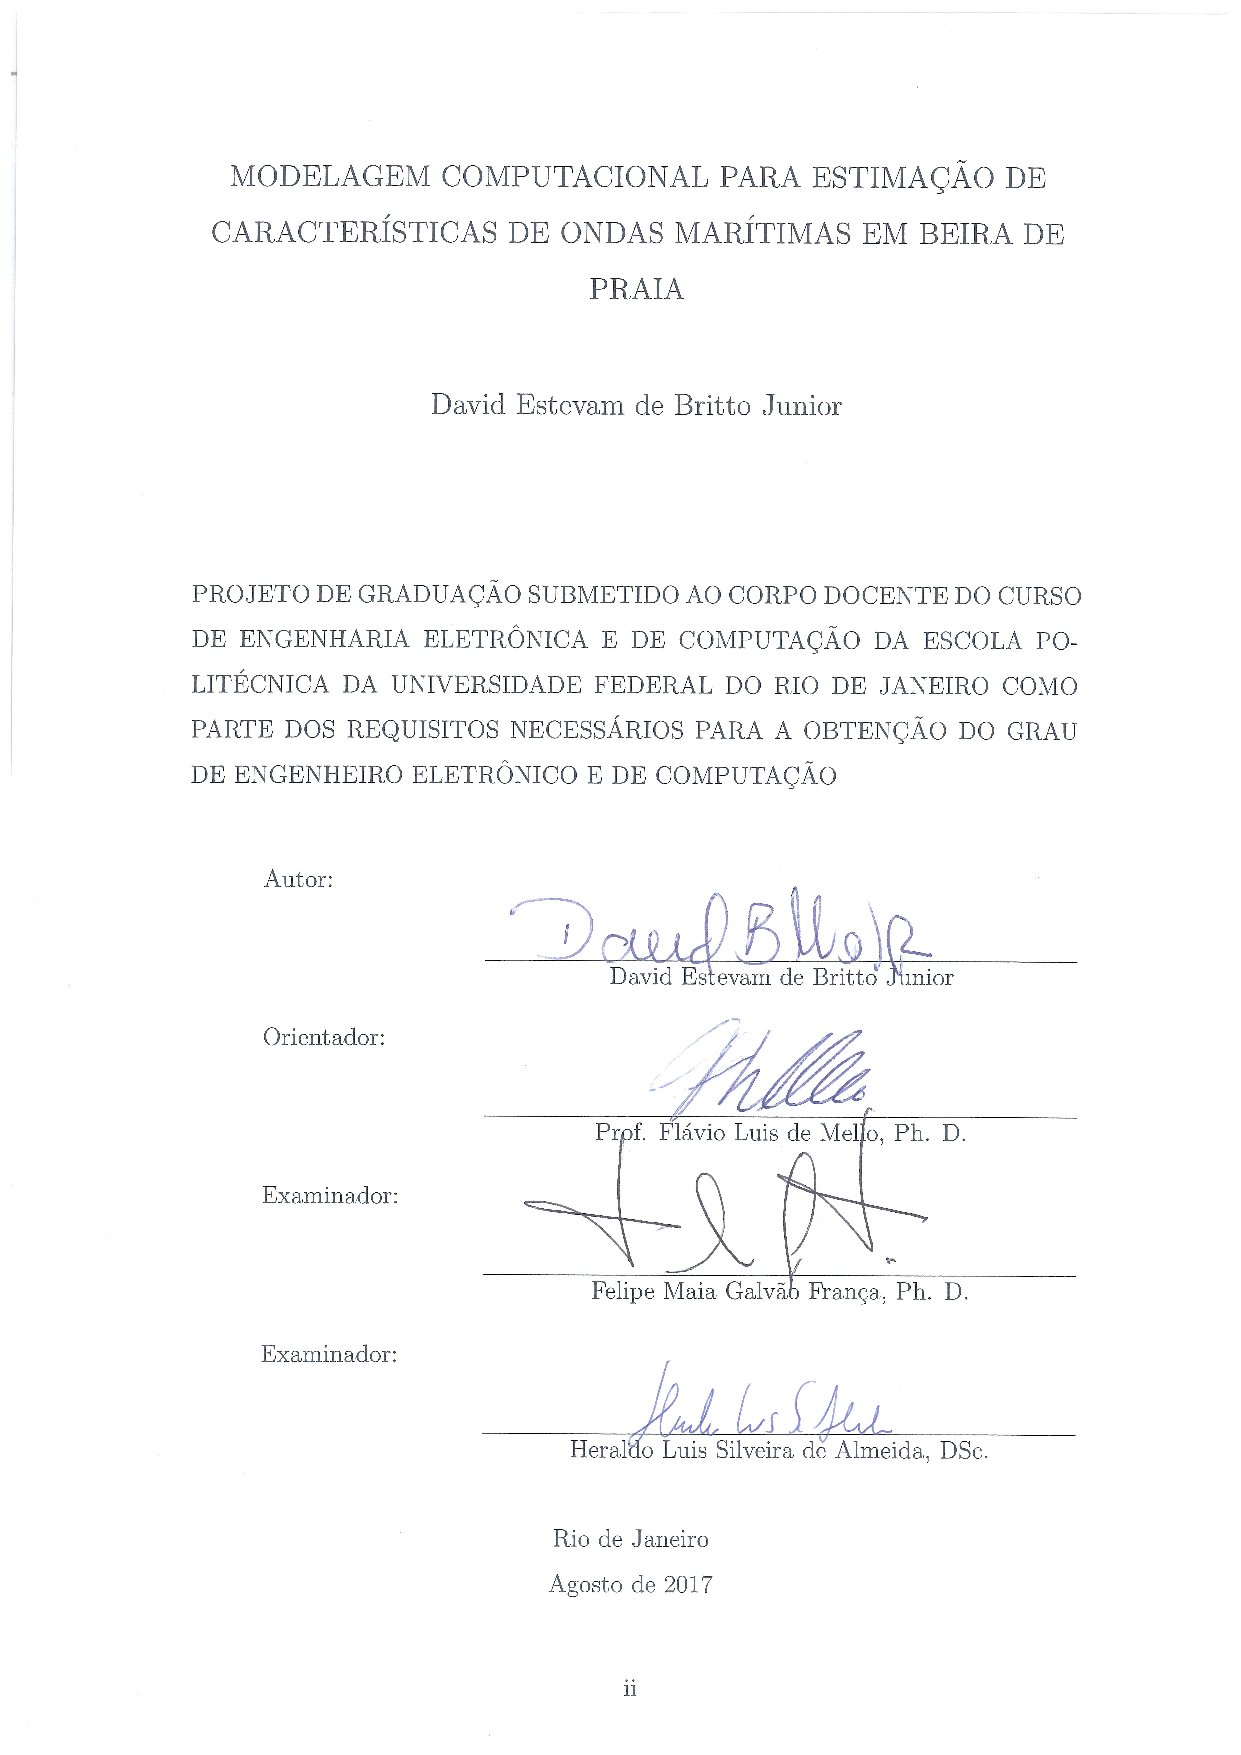
\includepdf{folha_assinatura_banca.pdf}

% \begin{figure}
%    \centering
%    \includefigure
% \end{figure}

% \begin{center}
% \large{MODELAGEM COMPUTACIONAL PARA ESTIMA��O DE CARACTER�STICAS DE ONDAS MAR�TIMAS EM BEIRA DE PRAIA}\\
%    \vspace{1cm}
% \large{David Estevam de Britto Junior}\\
% \end{center}
%    \vspace{2cm}
% PROJETO DE GRADUA��O SUBMETIDO AO CORPO DOCENTE DO CURSO DE ENGENHARIA ELETR�NICA E DE COMPUTA��O DA ESCOLA POLIT�CNICA DA UNIVERSIDADE FEDERAL DO RIO DE JANEIRO COMO PARTE DOS REQUISITOS NECESS�RIOS PARA A OBTEN��O DO GRAU DE ENGENHEIRO ELETR�NICO E DE COMPUTA��O   
   
%    \vspace{1cm}
% Autor:
%       \vspace{0.5cm}
%       \begin{flushright}
%          \parbox{10cm}{
%             \hrulefill

%             \vspace{-.375cm}
%             \centering{David Estevam de Britto Junior}

%             \vspace{0.1cm}
%          }
%       \end{flushright}
      
      
% Orientador:
%       \vspace{0.5cm}
%       \begin{flushright}
%          \parbox{10cm}{
%             \hrulefill

%             \vspace{-.375cm}
%             \centering{Prof. Fl\'avio Luis de Mello, Ph. D.}

%             \vspace{0.1cm}
%          }
%       \end{flushright}
      
% Examinador:
%       \vspace{0.5cm}
%       \begin{flushright}
%          \parbox{10cm}{
%             \hrulefill

%             \vspace{-.375cm}
%             \centering{Felipe Maia Galv�o Fran�a, Ph. D.}

%             \vspace{0.1cm}
%          }
%       \end{flushright}
      
% Examinador:
%       \vspace{0.5cm}
%       \begin{flushright}
%          \parbox{10cm}{
%             \hrulefill

%             \vspace{-.375cm}
%             \centering{Heraldo Luis Silveira de Almeida, DSc.}

%             \vspace{0.1cm}
%          }
%       \end{flushright}
      
                        
%       \vfill
      
      
% \begin{center}
% Rio de Janeiro

% Agosto de 2017
% \end{center}
